\documentclass[11pt]{beamer}
\usepackage{tikz, amsmath, hyperref, listings, courier, color, graphicx}
\usetikzlibrary{arrows.meta, arrows}

\mode<presentation> {
\usetheme{CambridgeUS}
}

\definecolor{mygreen}{rgb}{0,0.6,0}
\definecolor{mygray}{rgb}{0.5,0.5,0.5}
\definecolor{mymauve}{rgb}{0.58,0,0.82}

\lstset{
  basicstyle=\footnotesize\ttfamily,
  commentstyle=\color{mygreen},
  keywordstyle=\color{blue},
  stringstyle=\color{mymauve}
}

\setbeamertemplate{caption}{\raggedright\insertcaption\par}

\date{\today}

\title[6.905 Final Project]{The Typer Piper: Automating Data Structure Transformations Through Type Chaining} 

\author[Gruenstein \and Schneider]{
    Josh Gruenstein \and Martin Schneider
} 

\begin{document}

\begin{frame}
\titlepage 

\end{frame}

\begin{frame}
\frametitle{Contents} 
\tableofcontents 
\end{frame}

\section{Introduction} 
\begin{frame}{Motivation}
    \begin{figure}[h!]
        \centering

        \resizebox{10cm}{!} {
          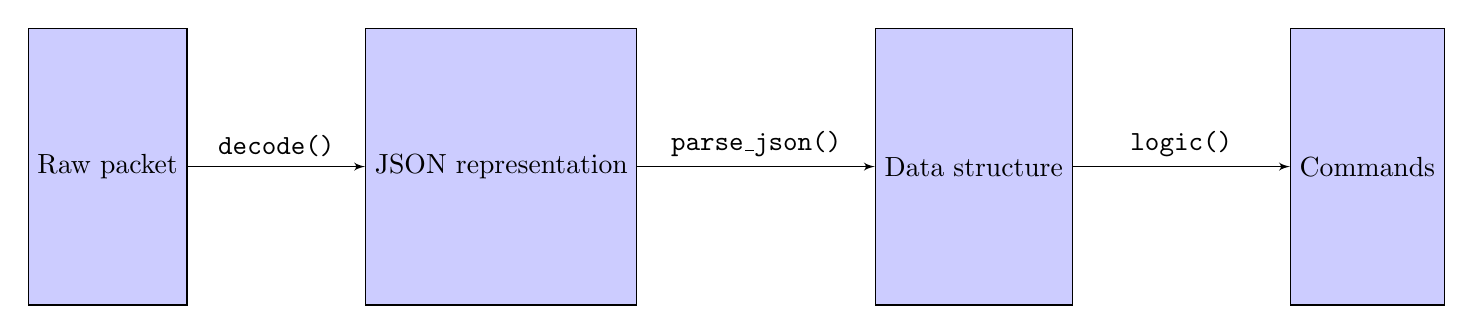
\begin{tikzpicture}[node distance=2.5cm,auto,>=latex']
	\tikzstyle{type}=[draw, fill=blue!20, minimum size=2em,minimum height=10em]
	\tikzstyle{init} = [pin edge={to-,thin,black}]

    \node [type] (a) {Raw packet};
    \node [type] (c) [right of=a, node distance=5cm] {JSON representation};
    \node [type] (d) [right of=c, node distance=6cm] {Data structure};
    \node [type] (e) [right of=d, node distance=5cm] {Commands};
    
    \path[->] (a) edge node {\texttt{decode()}} (c);
    \draw[->] (c) edge node {\texttt{parse\_json()}} (d);
    \draw[->] (d) edge node {\texttt{logic()}} (e);
\end{tikzpicture}
        }

        \caption{A type conversion diagram for a webserver.}
    \end{figure}
\end{frame}

\begin{frame}{Concept}
    \begin{itemize}
        \item Inference of type conversion flow
        \medskip
        \item Program superstructure writes itself
        \medskip
        \item Less code, less thinking, more good.
    \end{itemize}
\end{frame}

\section{Type System} 

\begin{frame}{Predicate Transformation Graph}
    \begin{figure}[h!]
        \centering

        \resizebox{6cm}{!} {
          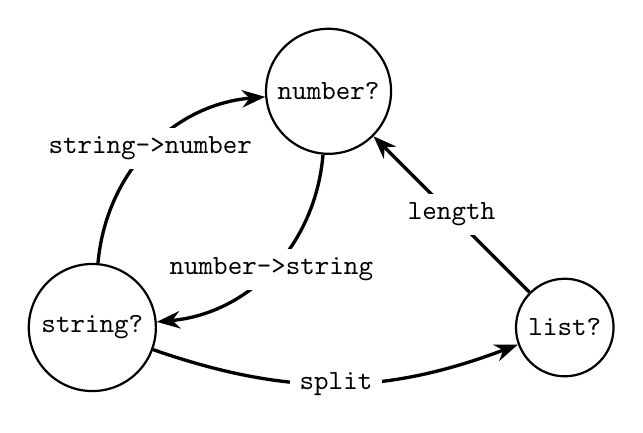
\begin{tikzpicture}
\begin{scope}[every node/.style={circle,thick,draw}]
    \node (A) at (0,0) {\texttt{string?}};
    \node (B) at (3,3) {\texttt{number?}};
    \node (C) at (6,0) {\texttt{list?}};
\end{scope}

\begin{scope}[>={Stealth[black]},
              every node/.style={fill=white},
              every edge/.style={draw=black,very thick}]
    \path [->] (A) edge[bend left=40] node {\texttt{string->number}} (B);
    \path [->] (B) edge[bend left=40] node {\texttt{number->string}} (A);
    \path [->] (C) edge node {\texttt{length}} (B);
    \path [->] (A) edge[bend right=20] node {\texttt{split}} (C);
\end{scope}
\end{tikzpicture}
        }

        \caption{An example predicate conversion graph.}
    \end{figure}
\end{frame}

\begin{frame}{Subtyping and Supertyping}
    \begin{figure}[h!]
        \centering

        \resizebox{!}{5cm} {
          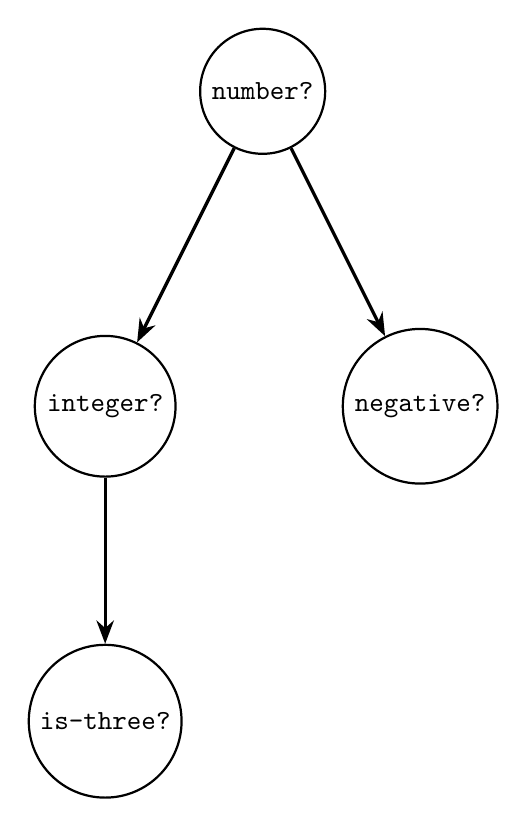
\begin{tikzpicture}
\begin{scope}[every node/.style={circle,thick,draw}]
    \node (A) at (0,0) {\texttt{number?}};
    \node (B) at (-2,-4) {\texttt{integer?}};
    \node (C) at (-2,-8) {\texttt{is-three?}};
    \node (D) at (2,-4) {\texttt{negative?}};
\end{scope}

\begin{scope}[>={Stealth[black]},
              every edge/.style={draw=black,very thick}]
    \path [->] (A) edge node {} (B);
    \path [->] (B) edge node {} (C);
    \path [->] (A) edge node {} (D);
    %\path [->] (C) edge node {\texttt{length}} (B);
    %\path [->] (A) edge[bend right=20] node {\texttt{split}} (C);
\end{scope}
\end{tikzpicture}
        }

        \caption{An example supertype tree.}
    \end{figure}

\end{frame}

\section{Search Engine}

\begin{frame}{Backtracking Search}
    \begin{itemize}
        \item Start at input predicate, take predicate transforms on edges to explore.
        \medskip
        \item Backtrack if dead end, and don't revisit predicates.
        \medskip
        \item \texttt{(string? number?)} $\overset{?}{\longrightarrow}$ \texttt{(string? string?)}
    \end{itemize}
\end{frame}

\begin{frame}{Compound Transformations}
    \begin{figure}[h!]
        \centering

        \resizebox{11cm}{!} {
          \texttt{(string? number?)} $\rightarrow \begin{bmatrix}
  \texttt{string?} \\
  \texttt{number?} \\
  \texttt{list?}
\end{bmatrix} \times \begin{bmatrix}
  \texttt{number?} \\
  \texttt{string?}
\end{bmatrix} \rightarrow \, \begin{matrix}
  \texttt{(string? number?)} \\
  \texttt{(string? string?)} \\
  \texttt{(number? number?)} \\
  \dotsc \\
  \texttt{(list? string?)}
\end{matrix}$

        }

        \caption{Transformations of \texttt{(string? number?)} using the example graph.}
    \end{figure}
\end{frame}

\begin{frame}{Joiner Transformations}

\texttt{person?} $\overset{?}{\longrightarrow}$ \texttt{(person:first? person:last?)}

\bigskip

\begin{enumerate}
    \medskip
    \item Find all possible compound targets using target and graph
    \medskip
    \item Filter those that can reach target
    \medskip
    \item Find path from input to each predicate in each compound
\end{enumerate}

\end{frame}

\section{Demos!}

\begin{frame}[fragile]
\frametitle{Simple example}

\begin{lstlisting}[language=lisp]
(register-predicate! list?)
(register-predicate! number?)
(register-predicate! string?)

(define (is-three? num) (eq? num 3))

(register-predicate! is-three?)
(register-super! is-three? number?)

(register-type-transform! list? number? length)
(register-type-transform! number? string? number->string)
(register-type-transform! string? number? string->number)

; (debug-transform number? string? 1)
; (debug-transform list? string? '(1 2 3))
; (debug-transform is-three? string? 3)

(debug-transform-to 3 string?)
\end{lstlisting}

\end{frame}

\begin{frame}{Pause for live demos!}

\begin{center} \Huge \textbf{DEMOS.} \end{center}

\end{frame}

\section{Discussion}

\begin{frame}{Programming as type conversion}
    \begin{figure}[h!]
        \centering

        \resizebox{10cm}{!} {
          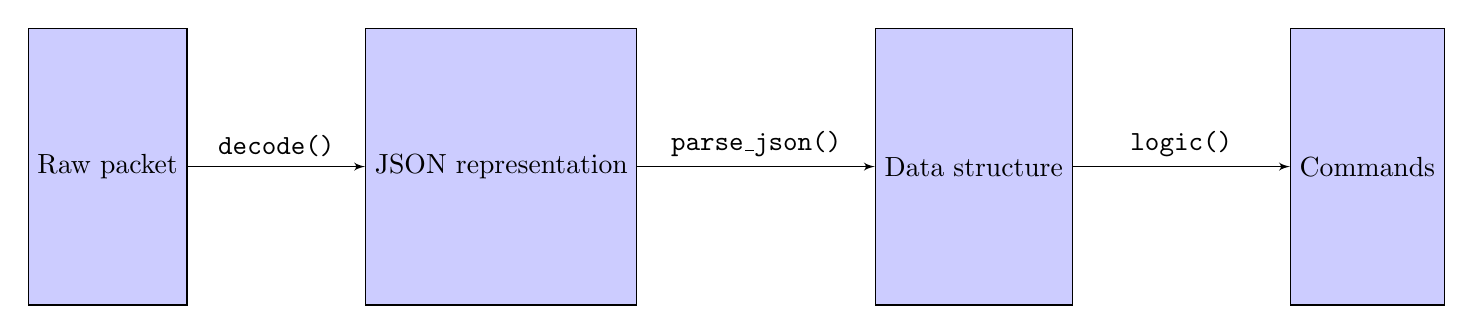
\begin{tikzpicture}[node distance=2.5cm,auto,>=latex']
	\tikzstyle{type}=[draw, fill=blue!20, minimum size=2em,minimum height=10em]
	\tikzstyle{init} = [pin edge={to-,thin,black}]

    \node [type] (a) {Raw packet};
    \node [type] (c) [right of=a, node distance=5cm] {JSON representation};
    \node [type] (d) [right of=c, node distance=6cm] {Data structure};
    \node [type] (e) [right of=d, node distance=5cm] {Commands};
    
    \path[->] (a) edge node {\texttt{decode()}} (c);
    \draw[->] (c) edge node {\texttt{parse\_json()}} (d);
    \draw[->] (d) edge node {\texttt{logic()}} (e);
\end{tikzpicture}
        }

        \caption{A type conversion diagram for a webserver.}
    \end{figure}
\end{frame}

\end{document}